% 首段缩进
\usepackage{indentfirst}

% 启用并隐藏超链接
\usepackage{hyperref}
\hypersetup{hidelinks}

% 调整行距
\usepackage{setspace}
\newcommand{\mysetspacing}{
    \setstretch{1.618}
}
\mysetspacing

% 段距
\setlength{\parskip}{0pt}

% 页面配置
\usepackage{geometry}
% 主布局
\newlength{\pw}
\newlength{\ph}
% A5 148*210
\setlength{\pw}{148mm}
\setlength{\ph}{210mm}

\newlength{\bleedlen}
\setlength{\bleedlen}{0mm}

\newlength{\ptop}
\newlength{\pbottom}
\newlength{\pinner}
\newlength{\pouter}
\newlength{\phsep}
\newlength{\pfskip}

\setlength{\ptop}{21mm}
\setlength{\pbottom}{21mm}
\setlength{\pinner}{22mm}
\setlength{\pouter}{13.5mm}
\setlength{\phsep}{.8\baselineskip}
\setlength{\pfskip}{2.2\baselineskip}
\addtolength{\pfskip}{-1em}
% 目录页布局
\newcommand{\tocgeo}{}
% 图片页布局
\newcommand{\picgeo}{\newgeometry{top=\bleedlen,bottom=\bleedlen,inner=\bleedlen,outer=\bleedlen}}
% 图片页布局
\newcommand{\buindinpicgeo}{}

\ifdefined\bleed
    \addtolength{\bleedlen}{3mm}
    \addtolength{\pw}{\bleedlen}
    \addtolength{\pw}{\bleedlen}
    \addtolength{\ph}{\bleedlen}
    \addtolength{\ph}{\bleedlen}
    \addtolength{\ptop}{\bleedlen}
    \addtolength{\pbottom}{\bleedlen}
    \addtolength{\pinner}{\bleedlen}
    \addtolength{\pouter}{\bleedlen}
    \renewcommand{\tocgeo}{\newgeometry{left=30mm,right=30mm,top=\ptop,bottom=\pbottom}}
\else
    \renewcommand{\tocgeo}{\newgeometry{left=27mm,right=27mm,top=\ptop,bottom=\pbottom}}
\fi

\newcommand{\charcount}{32}
\newcommand{\linecount}{25}

\newlength{\theight}
\setlength{\theight}{\linecount\baselineskip}
\addtolength{\theight}{1em}
\addtolength{\theight}{-\baselineskip}

\geometry{
    paperwidth=\pw,
    paperheight=\ph,
    top=\ptop,
    outer=\pouter,
    % inner=\pinner,
    % bottom=\pbottom,
    textwidth=\charcount\ccwd,
    textheight=\theight,
    headsep=\phsep,
    footskip=\pfskip
}

% 空白页
\newcommand{\blankpage}{
    \newpage
    \makebox{}
    \thispagestyle{empty}
    \newpage
}

% 空白段
\newcommand{\blankpar}{
    ~\
}

% 目录
% 目录参数
\counterwithout{section}{chapter}
\counterwithout{subsection}{section}
% 目录格式
\usepackage{titletoc}
% 章节符号
\newcommand{\myss}{\ssfont\S}
% 目录标题
\renewcommand{\contentsname}{
    目\quad 录
}
% 目录内标题格式
\titlecontents{part}
[0em]
{\vspace{1em}\Large\tocpart}
{}
{}
{\hspace{4mm}\pagenumberfont\contentspage}[\vspace{0.5em}]

\titlecontents{chapter}
[6mm]
{\vspace{0.3em}\large\tocchapter}
{\makebox[10mm][l]{\myss\hspace{0.1em}\normalsize\uppercase\expandafter{\romannumeral\thecontentslabel}}}
{}
{\hspace{4mm}\tocpage\large\contentspage}[\vspace{0.3em}]

\titlecontents{section}
[12mm]
{\tocsection}
{\tocsectlabel Ch \hspace{0.1em}\makebox[1em][c]{\thecontentslabel}\hspace{1em}}{}
{\hspace{5mm}\tocpage\contentspage}[\vspace{0.1em}]

\makeatletter
% 页码宽度
\renewcommand{\contentspage}[1][\thecontentspage]{\hb@xt@\@pnumwidth{#1\hfil}}
\renewcommand{\@pnumwidth}{9mm}
% 每章重置尾注编号
\@addtoreset{endnote}{chapter}  % Reset endnote numbering every new chapter
\@addtoreset{subsection}{section} % Reset subsection numbering every new section
\@addtoreset{section}{chapter} % Reset section numbering every new chapter
\@addtoreset{chapter}{part}  % Reset chapter numbering every new part
\makeatother
% 每页重置脚注编号
\usepackage{footnpag}

% 正文标题格式
\usepackage{titlesec}

\titleformat{\part}[display]{\centering\huge\partfont}{\thepart}{1.5pc}{\thispagestyle{empty}}
\titlespacing{\part}{0em}{.3\textheight}{0em}

\titleformat{\chapter}{\centering\Large\chapterfont}{}{0em}{}
\titlespacing{\chapter}{0em}{.5\baselineskip}{2\baselineskip}

\titleformat{\section}{\sectionfont}{Chapter~\thesection}{1em}{}
\titlespacing{\section}{2em}{1.4\baselineskip plus 2pt minus 2pt}{.5\baselineskip plus 2pt minus 2pt}

\titleformat{\subsection}{\subsectionfont}{0\thesubsection}{1em}{}
\titlespacing{\subsection}{2em}{.5\baselineskip plus 2pt minus 2pt}{.5\baselineskip plus 2pt minus 2pt}

\newcommand{\parttitle}{部名}

\usepackage{fancyhdr}
% 章节标记不出现chapter和序号
\renewcommand{\chaptermark}[1]{\markboth{\MakeUppercase{#1}}{}}
\renewcommand{\sectionmark}[1]{\markright{#1}}
% 去除页眉横线
\renewcommand{\headrulewidth}{0pt}
% 页脚溢出一点
\fancyfootoffset[RO,LE]{1.5em}
\fancypagestyle{mystyle}{
    \fancyhf{}
    \fancyhead[CE]{\headfont\mytitle}
    \fancyhead[CO]{\headfont\parttitle}
    \fancyfoot[CO]{\hfill\headfont\leftmark\qquad\rule[-4pt]{0.3pt}{20pt}\hspace{1.5em}}
    \fancyfoot[RO]{\pagenumberfont\thepage}
    \fancyfoot[LE]{\pagenumberfont\thepage}
    \fancyfoot[CE]{\hspace{1.5em}\rule[-4pt]{0.3pt}{20pt}\qquad\headfont\parttitle\hfill}
}
\fancypagestyle{plain}{
    \fancyhf{}
    \fancyfoot[CO]{\hfill\headfont\leftmark\qquad\rule[-4pt]{0.3pt}{20pt}\hspace{1.5em}}
    \fancyfoot[RO]{\pagenumberfont\thepage}
    \fancyfoot[LE]{\pagenumberfont\thepage}
    \fancyfoot[CE]{\hspace{1.5em}\rule[-4pt]{0.3pt}{20pt}\qquad\headfont\parttitle\hfill}
}
\usepackage{emptypage}

% 尾注
\usepackage{endnotes}
\renewcommand{\notesname}{注:}
\renewcommand{\enoteheading}{\section*{\notesname}\mbox{}\par\vskip-\baselineskip}
\renewcommand{\theendnote}{\roman{endnote}}

% 以下为非通用内容

% 故事完
\newcommand{\storyend}[1][完]{
    \nopagebreak
    \vspace{1.5\baselineskip}

    \blankpar

    \hfill \textbf{#1} \hspace{5em}

    \vspace{2.5\baselineskip}
}

\usepackage{changepage}
\renewenvironment{quotation}{
    \begin{adjustwidth}{2em}{2em}
        \quotefont
        }{
    \end{adjustwidth}
    \vspace{.5\baselineskip plus .5\baselineskip}
}
\renewenvironment{quote}{
    \vspace{0pt plus .3\baselineskip}

    \begin{adjustwidth}{2em}{2em}
        \quotefont}{
    \end{adjustwidth}

    \vspace{.3\baselineskip}
}


% 设置署名
\newcommand{\signature}{
    \vfill
    \setstretch{1.5}

    \begin{figure}[h]
        \hfill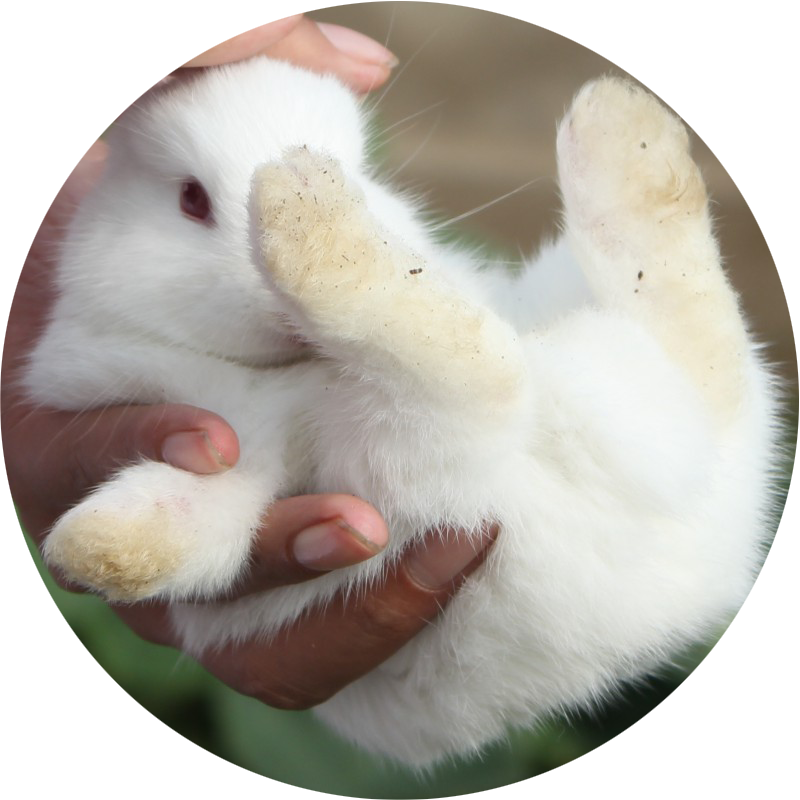
\includegraphics[width=2.8em]{headshot.png}\hspace{5.1em}
    \end{figure}

    \vspace{-1.5em}

    \hfill {\subsectionfont by\myauthor}\hspace{5em}

    \hfill {\subsectionfont \number\year.\number\month.\number\day} \hspace{4.8em}

    \vspace{2cm}
}

% 特殊符号和字体
\newcommand{\splitdot}{\dotfont ·}

\newcommand{\spell}[1]{{\spellfont #1}}

\newcommand{\tempsymbol}{{\tempfont℃}}

\newcommand{\chsline}{\makebox[2em]{——}}

% 章前注
\newcommand{\prenotes}[1]{
    \vspace{1.3\baselineskip}
    {\prenotefont #1}
    \vspace{.2\baselineskip}
}
% 章前注的参数
\newlength{\chapterblank}
\setlength{\chapterblank}{4.65\baselineskip}
\newlength{\prenoteblank}
\setlength{\prenoteblank}{1\baselineskip}
\newcommand{\doublelinechapter}{{\huge\vspace{-\baselineskip}}}

% 扉页
\newcommand{\mytitlepage}{
    \null
    \vfill
    \thispagestyle{empty}

    \begin{center}
        \Huge

        \titlefont

        {\mytitleen}

        \vspace{2mm}

        {\mytitle}

        \Large

        \vspace{60mm}

        {\cpfont\mycp}

        \vspace{2mm}

        {\signfont BY \myauthor}
    \end{center}

    \vfill

    \clearpage
}

% 尾页
\newcommand{\myendpage}{
    \newpage
    \ifodd\thepage
        \blankpage
    \fi

    \newpage

    \thispagestyle{empty}

    \

    \vfill

    \begin{minipage}{50mm}

        模板制作:兔子草

    \end{minipage}
    \vspace{5mm}
}

% 插入图片
\usepackage{graphicx}

% 让脚注不影响上文的行距
\usepackage[bottom]{footmisc}
% 脚注上方高度
\setlength{\footnotesep}{8pt}
% 脚注上方横线
\renewcommand{\footnoterule}{
    \kern -2pt
    \hrule width .25\textwidth height 0.5pt
    \kern 1.5pt
}

% section上方弹性换页
\usepackage{needspace}
\AddToHook{cmd/section/before}{\needspace{3\baselineskip}}

\let\origpart\part
\renewcommand*{\part}[2][]{
    \ifx\\#1\\% optional argument not present?
    \origpart{#2}
        \renewcommand*\parttitle{#2}
    \else
    \origpart[#1]{#2}
        \renewcommand*\parttitle{#1}
    \fi
    \mysetspacing
}
